\chapter{Verwendete Technologien}\label{cha:used-technologies}

\section{Message Queuing Telemetry Transport (MQTT)}\label{sec:mqtt}

Im Laufe der Arbeit werden folgende Begriffe erwähnt, welche hier erklärt werden:

\begin{enumerate}
    \item \textbf{Broker}:
    
    Ein Server, der alle Nachrichten von den Clients empfängt und diese dann an die entsprechenden Zielclients weiterleitet.

    \item \textbf{Topic}:
    
    In MQTT verweist das Wort Topic auf eine UTF-8-Zeichenfolge, die der Broker zum Filtern von Nachrichten für jeden verbundenen Client verwendet. Das Topic besteht aus einer oder mehreren Topiclevels. Jedes Topiclevel ist durch einen Slash getrennt.
    
    \item \textbf{Message}:
    
    Eine MQTT Message ist ein beliebiges Array von Bytes, welche an ein bestimmtes Topic gesendet werden.

    Wenn in dem Kapitel \ref{sec:own-libraries-mqtt} von einer MQTT Message geschrieben wird, dann steht dies für die Struktur, welche in der selben Library definiert wird.

    \item \textbf{Quality of Service (QoS)}:
    
    Das Quality of Service (QoS) Level ist eine Vereinbarung zwischen dem Absender einer Nachricht und dem Empfänger einer Nachricht, die die Zustellgarantie für eine bestimmte Nachricht definiert.
\end{enumerate}

\subsection{QoS}\label{sec:mqtt-qos}

In der nachstehenden Aufzählung werden die drei verschiedenen Arten von QoS näher erläutert, welche von der HiveMq Website\cite{hivemq} zusammengefasst wurden.

\begin{enumerate}
    \item \textbf{QoS 0 - maximal einmal}:
    Die minimale QoS-Stufe ist 0. Dieser Service-Level garantiert eine bestmögliche Lieferung. Es gibt keine Liefergarantie. Der Empfänger bestätigt den Empfang der Nachricht nicht und die Nachricht wird vom Absender nicht gespeichert und erneut gesendet. QoS-Stufe 0 wird oft als "fire and forget" bezeichnet und bietet die gleiche Garantie wie das zugrunde liegende TCP-Protokoll. 

    \begin{figure}[H]
        \begin{center}
            
\includegraphics[scale=0.8]{images/QoS-0.png}
            \caption{MQTT QoS 0 \cite{hivemq}}
        \end{center}
    \end{figure}

    \item \textbf{QoS 1 - mindestens einmal}:
    
    QoS Level 1 garantiert, dass eine Nachricht mindestens einmal an den Empfänger übermittelt wird. Der Absender speichert die Nachricht, bis er vom Empfänger ein Rückmeldung erhält, das den Empfang der Nachricht bestätigt. Es ist möglich, dass eine Nachricht mehrmals gesendet oder zugestellt wird.

    \begin{figure}[H]
        \begin{center}
            
\includegraphics[scale=0.8]{images/QoS-1.png}
            \caption{MQTT QoS 1 \cite{hivemq}}
        \end{center}
    \end{figure}

    \item \textbf{QoS 2 - genau einmal}:
    
    QoS 2 ist das höchste Servicelevel in MQTT. Diese Stufe garantiert, dass jede Nachricht nur einmal von den vorgesehenen Empfängern empfangen wird. QoS 2 ist die sicherste und langsamste Servicequalität. Die Garantie wird durch mindestens zwei request/response flows zwischen dem Sender und dem Empfänger bereitgestellt. 

    \begin{figure}[H]
        \begin{center}
            
\includegraphics[scale=0.8]{images/QoS-2.png}
            \caption{MQTT QoS 2 \cite{hivemq}}
        \end{center}
    \end{figure}
\end{enumerate}

\section{ESP-IDF Toolchain}\label{sec:esp-idf-toolchain}
Um die Toolchain verwenden zu können muss man sich in einem ESP-IDF Projektverzeichnis befinden. Hier kann ist es möglich, mit folgendem Befehl, den ESP zu konfigurieren:

\begin{verbatim}
    idf.py menuconfig
\end{verbatim}

Dieser Befehl startet folgendes Konfigurationsprogramm:
\begin{figure}[H]
    \begin{center}
        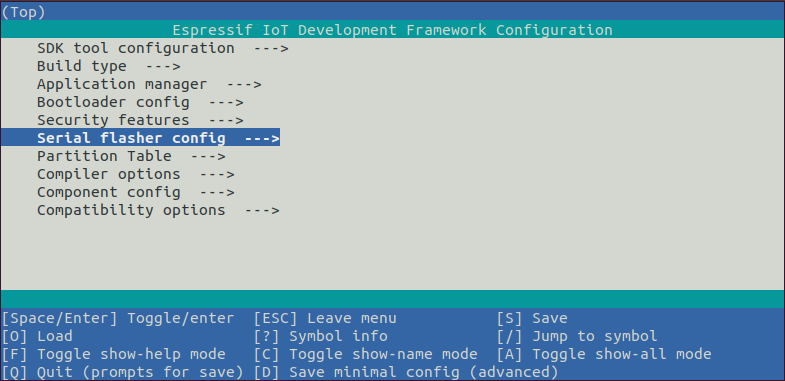
\includegraphics[scale=0.5]{images/menuconfig.png}
        \caption{menuconfig \cite{menuconfig_picture}}
    \end{center}
\end{figure}
Dieses Konfigurationsprogramm wird verwendet, um projektspezifische Variablen zu setzen, wie zB
\begin{itemize}
    \item Netzwerkname
    \item Netzwerkpasswort
    \item Takt des Prozessors
    \item Parition Table Variante
    \item \dots und viele mehr
\end{itemize}


%TODO beispiele für projbuild
\subsection{KConfig.projbuild}\label{sec:esp-idf-projbuild}
Sind die, von Espressif, zur Verfügung gestellten Menüs nicht genug, so ist es möglich eine \textbf{KConfig.projbuild} Datei anzulegen. Mit dieser Datei ist es möglich neue Top-Level Menüeinträge und Untermenüeinträge zu generieren. Dies wird benötigt, da in der standarmäßigen \textbf{menuconfig} nur der Großteil der gebrauchten Konfigurations-Felder zur Verfügung gestellt werden.

\subsection{Kompilieren}
Damit die fertigen Espressif Beispiele auf einem Dual-Core ESP funktionieren, muss sich dieser im Single-Core Modus befinden.

Ist das Projekt richtig konfiguriert kann es mit folgendem Befehl gebuildet werden:
\begin{verbatim}
    idf.py build
\end{verbatim}

Mit diesem Befehl wird die Anwendung kompiliert sowie der Bootloader und der Partition Table erstellt.

Sollten beim Kompilieren Fehler auftreten, so werden diese in der Konsole ausgegeben.

\subsection{Flashen}
Verläuft das Kompilieren Fehlerfrei, kann das Programm mit diesem Befehl auf den ESP geflasht werden:
\begin{verbatim}
    idf.py flash
\end{verbatim}

Sollte es ein Problem beim Flashen geben, liegt dies häufig an einem kaputten USB-Kabel.

Zumeist ist ein Problem beim Flashen auf ein kaputtes USB-Kabel zurückzuführen.

\subsubsection{IDF Monitor}\label{sec:monitor}
Der IDF-Monitor ist ein serielles Terminalprogramm, das serielle Daten zum und vom seriellen Anschluss des Zielgeräts weiterleitet.

Ist das Programm bereits auf dem ESP kann es mit folgendem Befehl auf dem IDF Monitor, überprüft werden.

\begin{verbatim}
    idf.py monitor
\end{verbatim}

Mit dem nachstehenden Befehl kann das Programm gebuildet, geflasht und upgeloadet werden. Dies erspart den Aufwand jeden Befehl einzeln einzugeben.

\begin{verbatim}
    idf.py flash monitor
\end{verbatim}

\section{Nodejs}\label{sec:nodejs}

Nodejs ist eine Laufzeit die auf der Javascript Engine von Chrome aufbaut. Nodejs wurde für das Backend des OTA Servers verwendet.

\subsection{Warum Nodejs?}
%TODO umändern
bei Vergleich Aufgabe erwähnen

Bei der Überlegung welche Sprache bzw. welches Framework für das Backend gewählt wird, war die Entscheidung sehr leicht.
Die Anforderungen des OTA Servers sind sehr einfach. Der Server dient nur zur Bereitstellung der Firmwares und beschreibende Informationen über die Firmwares selber.
Da dies nicht CPU intensiv ist sondern I/O intensiv, wurde in diesem Fall Nodejs gewählt.

\subsection{Event Loop}

\subsubsection{Was ist der Event Loop?}

Nodejs selber ist single-threaded deswegen ist der Event Loop einer der wichtigsten Bestandteile von Nodejs.
Der Event Loop erlaubt es nicht-blockenede I/O Operationen durchzuführen. Dies passiert durch die Abladung auf den Kernel von so vielen Operationen wie möglich.
\newline
\newline
Die meisten modernen Kernels sind multi-threaded. Das bedeutet, dass sie mehrere Operationen im Hintergrund unterstützen.

\subsubsection{Wie funktioniert der Event Loop?}

\begin{figure}[H]
    \begin{center}
        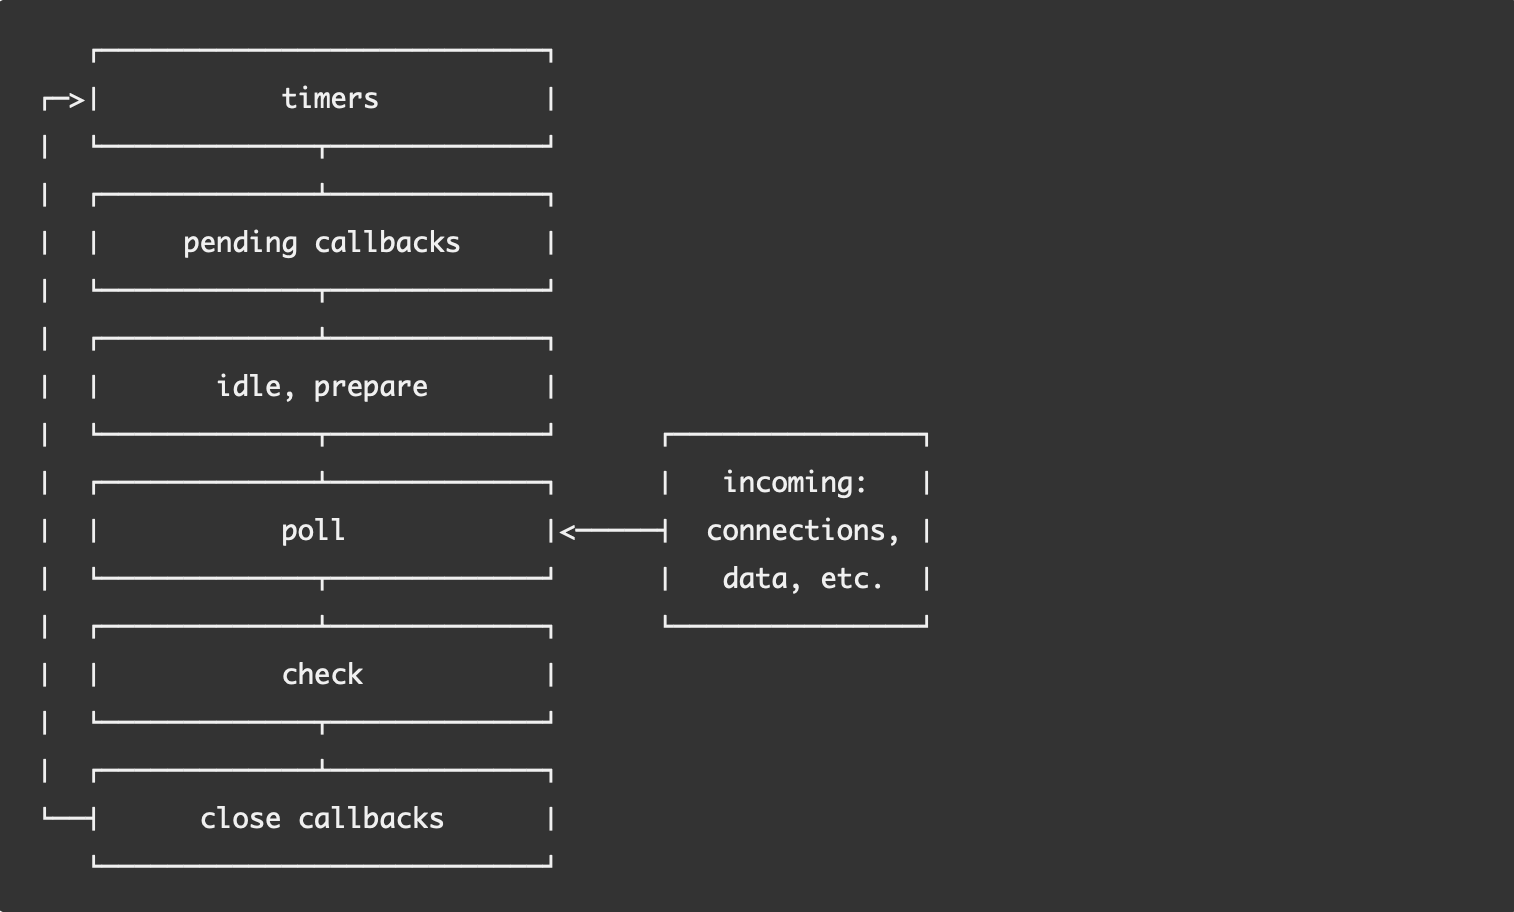
\includegraphics[scale=0.5]{images/nodejs_event_loop.png}
        \caption{Nodejs Event Loop \cite{nodejs_event_loop}}
    \end{center}
\end{figure}

Jeder Block im obigen Bild wird als Phase bezeichnet.
Jede Phase verfügt über eine First-In-First-Out-Warteschlange (FIFO-Warteschlange) mit auszuführenden Rückrufen. 
Während jede Phase auf ihre Weise etwas Besonderes ist, führt sie im Allgemeinen,
wenn die Ereignisschleife in eine bestimmte Phase eintritt, alle für diese Phase spezifischen Operationen aus und führt dann Rückrufe in der Warteschlange dieser Phase aus, 
bis die Warteschlange erschöpft ist oder die maximale Anzahl von Rückrufen ausgeführt hat. 
Wenn die Warteschlange erschöpft ist oder das Rückruflimit erreicht ist, wechselt die Ereignisschleife zur nächsten Phase und so weiter.
\newline
\newline
Da für jeden dieser Vorgänge möglicherweise mehr Vorgänge geplant werden und neue Ereignisse, 
die in der Abfragephase verarbeitet wurden, vom Kernel in die Warteschlange gestellt werden, 
können Abrufereignisse in die Warteschlange gestellt werden, während Abrufereignisse verarbeitet werden. 
Infolgedessen können lange laufende Rückrufe dazu führen, dass die Abfragephase viel länger als der Schwellenwert eines Timers läuft. 

\subsubsection{Phasen}

\begin{itemize}
    \item \textbf{timers:} In dieser Phase werden von setTimeout () und setInterval () geplante Rückrufe ausgeführt.
    \item \textbf{pending callbacks:} führt I/O Callbacks aus, die auf die nächste Iteration verschoben werden
    \item \textbf{idle, prepare:} wird nur intern verwendet
    \item \textbf{poll:} neue I/O Events abrufen; I/O bezogene Callbacks ausführen (fast alle mit Ausnahme von schließ Callbacks, die von Timers geplant werden, und setImmediate ()); Der Knoten wird hier gegebenenfalls blockiert
    \item \textbf{check:} setImmediate() Callbacks werden hier ausgeführt
    \item \textbf{close callbacks:} schließ Callbacks werden ausgeführt
\end{itemize}

Zwischen jedem Durchlauf des Event Loops prüft Nodejs, ob es auf asynchrone I/O oder Timer wartet, und fährt sauber herunter, wenn keine vorhanden sind.

\cite[Zitiert von der offizielen Nodejs Website]{nodejs_event_loop_how_does_it_work}

\section{Platform IO}\label{sec:platformio}

PlatformIO ist ein fortschrittliches und äußerst vielseitiges Ökosystem für die IoT-Entwicklung, das eine IDE, ein Build-System, einen Unified Debugger und einen Bibliotheksmanager umfasst. Es bietet Unterstützung für mehr als 550 Entwicklungsboards, mehr als 25 Entwicklungsplattformen und mehr als 10 nützliche Frameworks. Die PlatformIO IDE ist ein plattformübergreifendes Dienstprogramm für die schnelle berufliche Weiterentwicklung mit integriertem C / C++ - Intelligent Code Completion, Smart Code Linter und erweitertem Serial Port Monitor. PlatformIO kann auch in die gängigen IDEs und kontinuierlichen Integrationssysteme integriert werden, um die Zeit für die Bereitstellung von IoT-Anwendungen zu verkürzen.\cite{platformio_about_us}

PlatformIO ist in reinem Python geschrieben und hängt nicht von zusätzlichen Bibliotheken / Tools eines Betriebssystems ab. So kann man mit PlatformIO auf Windows, Macintosh und Linux arbeiten.

\section{Docker}\label{sec:docker}

Docker ist ein Open-Source-Projekt zur Automatisierung der Bereitstellung von Anwendungen als tragbare Container, die überall ausgeführt werden können. 

\subsection{Docker vs. Virtuelle Maschinen}\label{sec:docker-vm}

\subsubsection{Virtuelle Maschinen}

\begin{figure}[H]
    \begin{center}
        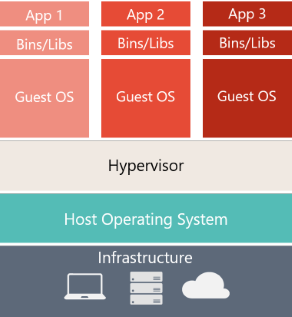
\includegraphics[scale=0.8]{images/docker-vm.png}
        \caption{Docker Virtuelle Maschine (Quelle: eigene Darstellung)}
    \end{center}
\end{figure}

Zu den virtuellen Maschinen gehören die Anwendung, die erforderlichen Bibliotheken oder Binärdateien sowie ein vollständiges Gastbetriebssystem. Die vollständige Virtualisierung erfordert mehr Ressourcen als die Containerisierung. \cite{docker}

\subsubsection{Docker}

\begin{figure}[H]
    \begin{center}
        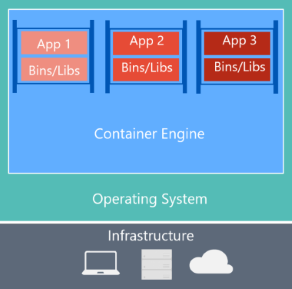
\includegraphics[scale=0.8]{images/docker.png}
        \caption{Docker (Quelle: eigene Darstellung)}
    \end{center}
\end{figure}

Container enthalten die Anwendung und alle ihre Abhängigkeiten. Sie teilen den Betriebssystemkern jedoch mit anderen Containern und werden als isolierte Prozesse im Benutzerbereich des Host-Betriebssystems ausgeführt. (Außer in Hyper-V-Containern, in denen jeder Container innerhalb einer speziellen virtuellen Maschine pro Container ausgeführt wird.) \cite{docker}

\subsection{Begriffe}\label{docker-terminology}

Im Laufe der Arbeit werden folgende Begriffe erwähnt:

\begin{enumerate}
    \item \textbf{Container}:
    
    Ein Container ist eine Instanz eines Images. Er repräsentiert die Ausführung einer einzelnen Anwendung, eines Prozesses oder eines Dienstes. 

    \item \textbf{Image}:
    
    Ein Image ist ein Paket mit allen Abhängigkeiten und Informationen, die zum Erstellen eines Containers erforderlich sind. Ein Image enthält alle Abhängigkeiten (z. B. Frameworks) sowie die Bereitstellungs- und Ausführungskonfiguration, die von einer Container-Laufzeit verwendet werden soll. 

    \item \textbf{Volume}:
    
    Ein Volume ist ein beschreibbares Dateisystem, das der Container verwenden kann. Da Images schreibgeschützt sind fügen Volumes eine beschreibbare Ebene über dem Image hinzu, sodass die Programme Zugriff auf ein beschreibbares Dateisystem haben. 

    \item \textbf{Network}:

    In einem Docker Network können Container auf sich gegenseitig mittels ihren Namen referenziern. Dies erleichtert das miteinander Arbeiten von verschiedenen Containern.
\end{enumerate}

\section{Docker Compose}\label{sec:docker-compose}

Docker-compose ist ein Tool zum Definieren und Ausführen von Docker-Anwendungen mit mehreren Containern. Mit Compose wird eine YAML-Datei verwendet, um die Dienste von Anwendung zu konfigurieren. Anschließend werden alle Dienste mit einem einzigen Befehl erstellt und gestartet. \cite{docker_compose_description}

\subsection{Docker Compose Beispiel}

\begin{figure}[H]
    \begin{center}
        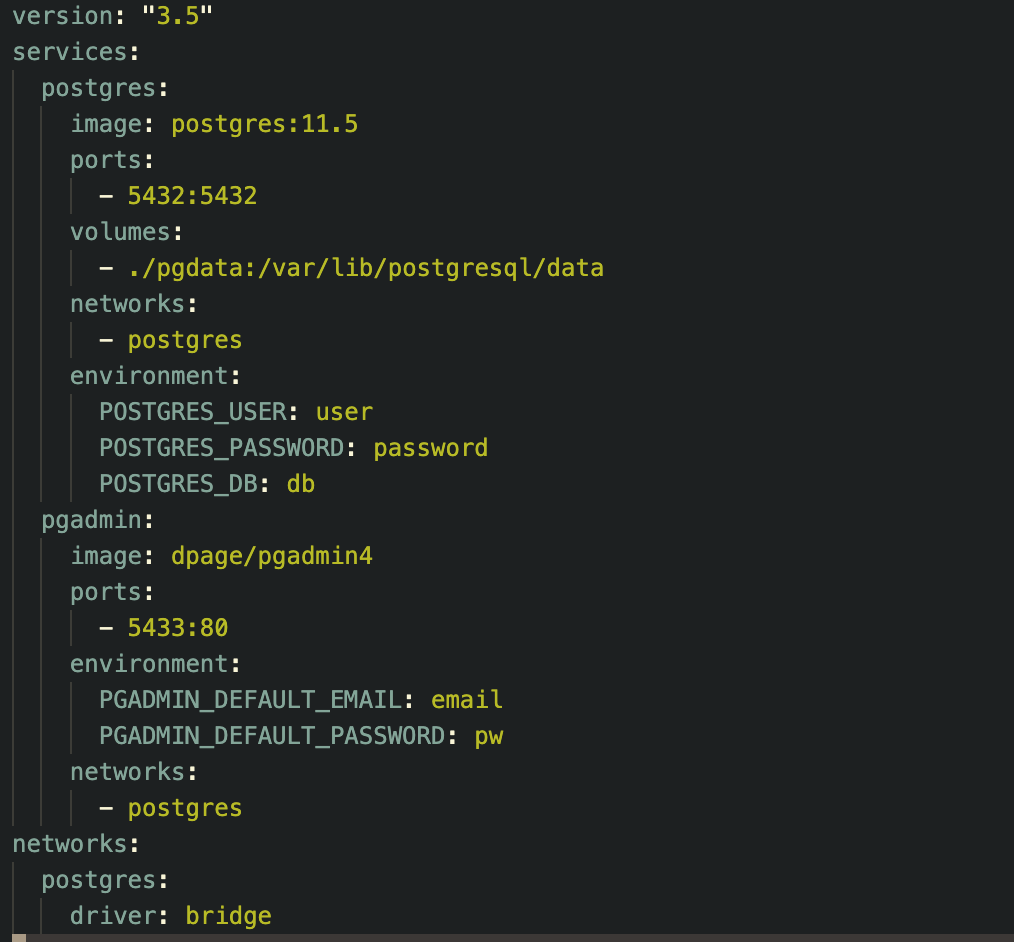
\includegraphics[scale=0.8]{images/docker_compose_example.png}
        \caption{Docker Compose Beispiel (Quelle: eigene Darstellung)}
        \label{abb:docker-compose-example}
    \end{center}
\end{figure}

In der obigen Abbildung kann man das docker-compose.yml file von dem OTA Server sehen.

Die Struktur eines docker-compose files ist im Normalfall immer gleich. Am Anfang definiert man welche Version des Standards man verwendet und anschließend die verschiedenen Dienste. Der OTA Server benötigt nur 2 Dienste:

\begin{enumerate}
    \item Postgres
    \item PgAdmin4
\end{enumerate}

In Abbildung \ref{abb:docker-compse-example} wird ein Netzwerk explizit erstellt. Es ist auch möglich das Netwerk implizit zu erstellen, indem man den networks Bereich von ganz unten entfernt.

\subsubsection{Postgres}

Datenbank für die Speicherung von den Informationen über die verschieden Firmwares die gerade auf dem Server hochgeladen sind.

Die Datenbank braucht irgendeinen Weg um mit der Außenwelt kommunizieren zu können, deswegen wird der interne Port 5432 auf den externen Port 5432 geleitet.

Damit die Absicherung der Datenbank leicht verläuft wird ein Volume für die Datenbank erstellt, worin sich die Daten der Datenbank befinden. In dieser docker-compose Datei wird das Volume implizit erstellt. 

Man kann es auch explizit erstellen wie folgt:

\begin{verbatim}
    volumes:
        pgdata:
\end{verbatim}

Mit den Umgebungsvariablen kann man die Standardwerte überschreiben. Die Datenbank hat in der obigen Abbildung den Benutzer \textit{user} mit dem Passwort \textit{password} und der default Datenbank \textit{db}.

\subsubsection{PgAdmin4}

PgAdmin4 ist eine web-basierte Benutzeroberfläche für Postgres.

Sie ist die PhpMyAdmin Oberfläche in der postgres Welt.

Die Software binded automatisch auf den Port 80, was für Entwicklungszwecke sehr unpraktisch ist, da Port 80 auf Ubuntu zum Beispiel Adminrechte benötigt. Deswegen wird der interne Port 80 auf den externen Port 5433 umgeleitet.

Mit den Umgebungsvariablen \textit{PGADMIN\_DEFAULT\_EMAIL} und 
\textit{PGADMIN\_DEFAULT\_PASSWORD} werden die default Logindaten für PgAdmin4 definiert. 
\pagebreak

\section{Utility lib Köck}\label{sec:utility-lib-koeck}
Dies ist Professor Köcks Library Sammlung, welche er persönlich verfasste. Sämtliche Technologien, welche durch die Libraries untersützt werden, sind in folgender Abbildung zu sehen.

\begin{figure}[H]
    \begin{center}
        \includegraphics[scale=0.9]{images/utility_lib_köck_own.PNG}
        \caption{Technologien Utility lib (Quelle: eigene Darstellung)}
    \end{center}
\end{figure}

\pagebreak
Dazu sind folgende Sensor Libraries ebenfalls enthalten:

\begin{figure}[H]
    \begin{center}
        \includegraphics[scale=0.9]{images/utility_lib_köck_sensors.PNG}
        \caption{Sensoren und Aktoren Utility lib (Quelle: eigene Darstellung)}
    \end{center}
\end{figure}

Im Laufe der Arbeit erfolgte ein Umstieg auf die offiziellen Espressif Libraries, da Professor Köcks Library Sammlung aufgrund fehlender Funktionalität für diese Diplomarbeit nicht mehr geeignet war.

Da alle Espressif Libraries in der Programmiersprache C geschrieben sind, ist es nicht möglich diese mit den Libraries von Professor Köck gleichzeitig zu verwenden. Da diese in C++ geschrieben sind und die Espressif Libraries Funktionen aus C verwenden, welche in C++ nicht unterstützt werden. Um Kompatibilität herzustellen ist es bei jeder Anwendung notwendig die Espressif Libraries anzupassen.